\documentclass[11pt]{article}
\usepackage{mathtools}
\usepackage{mdframed}
\usepackage{fullpage}
\usepackage{amsfonts}
\usepackage{tikz}
\usetikzlibrary{automata, positioning}



%edit this for each class
\newcommand\name{John Vincent}
\newcommand\classname{Com S 311}
\newcommand\assignment{Homework 3}



\newcounter{excounter}
\setcounter{excounter}{1}
\newcommand\question[2]{\vskip 1em  \noindent\textbf{\arabic{excounter}\addtocounter{excounter}{1}.} \emph{#1} \noindent#2}


% You can also erase this if you do not have package fancyhdr
% Fancy footnote.........
\usepackage{fancyhdr}  %% If it does not work with your latex installation, you may just delete this...
\pagestyle{fancy}
\usepackage{lastpage}
\rfoot{\name, page \thepage/\pageref{LastPage}}
\cfoot{}
\rhead{}
\lhead{}
\renewcommand{\headrulewidth}{0pt}
\renewcommand{\footrulewidth}{0pt}
\DeclarePairedDelimiter\ceil{\lceil}{\rceil}
\DeclarePairedDelimiter\floor{\lfloor}{\rfloor}



\begin{document}


  {\bf \classname \hspace{1cm} \assignment\hfill \name}
  \vskip 2em


  \question{}\\
  \indent a)\\
  \begin{center}
    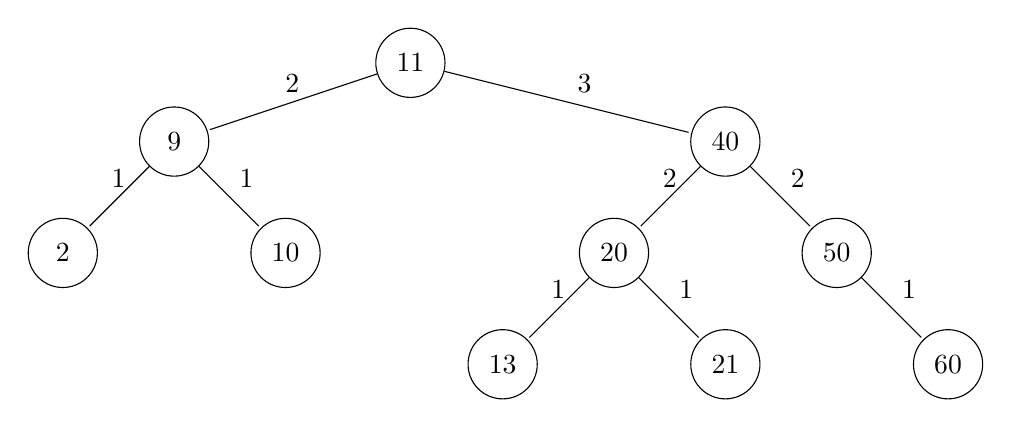
\begin{tikzpicture}[shorten >=1pt,node distance=2cm,on grid,auto]
      \node[state] (q_0) {$11$};
      \node[state] (q_1) [below right = 1cm and 4cm of q_0] {$40$};
      \node[state] (q_2) [below left of= q_1] {$20$};
      \node[state] (q_3) [below left of=q_2] {$13$};
      \node[state] (q_4) [below right of=q_2] {$21$};
      \node[state] (q_5) [below right of=q_1] {$50$};
      \node[state] (q_6) [below right of=q_5] {$60$};
      \node[state] (q_7) [below left=1cm and 3cm of q_0] {$9$};
      \node[state] (q_8) [below left of=q_7] {$2$};
      \node[state] (q_9) [below right of=q_7] {$10$};

      \path (q_0) edge node {3} (q_1)
            (q_0) edge node [above] {2} (q_7);
      \path (q_1) edge node [above] {2} (q_2)
            (q_1) edge node {2} (q_5);
      \path (q_2) edge node [above] {1} (q_3)
            (q_2) edge node {1} (q_4);
      \path (q_5) edge node {1} (q_6);
      \path (q_7) edge node [above] {1} (q_8)
            (q_7) edge node {1} (q_9);
    \end{tikzpicture}
  \end{center}

  \indent b) the tree is already balanced as all left and right children differ in
  height by at most 1.

  \indent c)

  \question{}\\
  \begin{quote}
    if the element $E$ is smaller that $2^{\ell-2}-1$ elements than it is bigger
    than at least $n$ elements.
    \begin{align*}
      n &= 2^{\ell} - 1 - (2^{\ell-2} -1)\\
      &= 2^{\ell}  - \frac{2^{\ell}}{4}\\
      &= \frac{3}{4}
    \end{align*}
  \end{quote}

\end{document}
